\documentclass{beamer}

\usepackage{algorithm}
\usepackage{algpseudocode}
\usepackage{mathtools}

\usefonttheme{serif}
\usepackage{dsfont}
\setbeamersize{text margin left=5pt, text margin right=5pt}

\newcommand{\bgk}[1]{\boldsymbol{#1}}

\newcommand{\bzero}{\bgk{0}}
\newcommand{\bone}{\bgk{1}}

\newcommand{\balpha}{\bgk{\alpha}}
\newcommand{\bnu}{\bgk{\nu}}
\newcommand{\bbeta}{\bgk{\beta}}
\newcommand{\bxi}{\bgk{\xi}}
\newcommand{\bgamma}{\bgk{\gamma}} 
\newcommand{\bo}{\bgk{o }}
\newcommand{\bdelta}{\bgk{\delta}}
\newcommand{\bpi}{\bgk{\pi}}
\newcommand{\bepsilon}{\bgk{\epsilon}} 
\newcommand{\bvarepsilon}{\bgk{\varepsilon}} 
\newcommand{\brho}{\bgk{\rho}}
\newcommand{\bvarrho}{\bgk{\varrho}}
\newcommand{\bzeta}{\bgk{\zeta}}
\newcommand{\bsigma}{\bgk{\sigma}}
\newcommand{\boldeta}{\bgk{\eta}}
\newcommand{\btay}{\bgk{\tau}}
\newcommand{\btheta}{\bgk{\theta}}
\newcommand{\bvertheta}{\bgk{\vartheta}}
\newcommand{\bupsilon}{\bgk{\upsilon}}
\newcommand{\biota}{\bgk{\iota}}
\newcommand{\bphi}{\bgk{\phi}}
\newcommand{\bvarphi}{\bgk{\varphi}}
\newcommand{\bkappa}{\bgk{\kappa}}
\newcommand{\bchi}{\bgk{\chi}}
\newcommand{\blambda}{\bgk{\lambda}}
\newcommand{\bpsi}{\bgk{\psi}}
\newcommand{\bmu}{\bgk{\mu}}
\newcommand{\bomega}{\bgk{\omega}}

\newcommand{\bA}{\bgk{A}}
\newcommand{\bDelta}{\bgk{\Delta}}
\newcommand{\bLambda}{\bgk{\Lambda}}
\newcommand{\bSigma}{\bgk{\Sigma}}
\newcommand{\bOmega}{\bgk{\Omega}}
\newcommand{\bPsi}{\bgk{\Psi}}

\newcommand{\bvec}[1]{\mathbf{#1}}

\newcommand{\va}{\bvec{a}}
\newcommand{\vb}{\bvec{b}}
\newcommand{\vc}{\bvec{c}}
\newcommand{\vd}{\bvec{d}}
\newcommand{\ve}{\bvec{e}}
\newcommand{\vf}{\bvec{f}}
\newcommand{\vg}{\bvec{g}}
\newcommand{\vh}{\bvec{h}}
\newcommand{\vi}{\bvec{i}}
\newcommand{\vj}{\bvec{j}}
\newcommand{\vk}{\bvec{k}}
\newcommand{\vl}{\bvec{l}}
\newcommand{\vm}{\bvec{m}}
\newcommand{\vn}{\bvec{n}}
\newcommand{\vo}{\bvec{o}}
\newcommand{\vp}{\bvec{p}}
\newcommand{\vq}{\bvec{q}}
\newcommand{\vr}{\bvec{r}}
\newcommand{\vs}{\bvec{s}}
\newcommand{\vt}{\bvec{t}}
\newcommand{\vu}{\bvec{u}}
\newcommand{\vv}{\bvec{v}}
\newcommand{\vw}{\bvec{w}}
\newcommand{\vx}{\bvec{x}}
\newcommand{\vy}{\bvec{y}}
\newcommand{\vz}{\bvec{z}}

\newcommand{\vA}{\bvec{A}}
\newcommand{\vB}{\bvec{B}}
\newcommand{\vC}{\bvec{C}}
\newcommand{\vD}{\bvec{D}}
\newcommand{\vE}{\bvec{E}}
\newcommand{\vF}{\bvec{F}}
\newcommand{\vG}{\bvec{G}}
\newcommand{\vH}{\bvec{H}}
\newcommand{\vI}{\bvec{I}}
\newcommand{\vJ}{\bvec{J}}
\newcommand{\vK}{\bvec{K}}
\newcommand{\vL}{\bvec{L}}
\newcommand{\vM}{\bvec{M}}
\newcommand{\vN}{\bvec{N}}
\newcommand{\vO}{\bvec{O}}
\newcommand{\vP}{\bvec{P}}
\newcommand{\vQ}{\bvec{Q}}
\newcommand{\vR}{\bvec{R}}
\newcommand{\vS}{\bvec{S}}
\newcommand{\vT}{\bvec{T}}
\newcommand{\vU}{\bvec{U}}
\newcommand{\vV}{\bvec{V}}
\newcommand{\vW}{\bvec{W}}
\newcommand{\vX}{\bvec{X}}
\newcommand{\vY}{\bvec{Y}}
\newcommand{\vZ}{\bvec{Z}}

\usepackage{subcaption}
\newcommand{\bitem}{\item[$\bullet$]}

\usepackage{xcolor}
\usepackage[utf8]{inputenc}
\DeclareFontEncoding{LS1}{}{}
\DeclareFontSubstitution{LS1}{stix}{m}{n}
\DeclareSymbolFont{symbols2}{LS1}{stixfrak} {m} {n}
\DeclareMathSymbol{\operp}{\mathbin}{symbols2}{"A8}
\setbeamertemplate{navigation symbols}{}

\usepackage{lipsum}

\newtheorem{proposition}[theorem]{Proposition}

\newcommand\blfootnote[1]{%
  \begingroup
  \renewcommand\thefootnote{}\footnote{#1}%
  \addtocounter{footnote}{-1}%
  \endgroup
}

\addtobeamertemplate{navigation symbols}{}{%
    \usebeamerfont{footline}%
    \usebeamercolor[fg]{footline}%
    \hspace{1em}%
    \insertframenumber/\inserttotalframenumber
}

\title{
Multi-linear Algebra\\
-- Hierarchical Tucker Decomposition --\\
Lecture 19
}
%\subtitle{Mathematical framework, existence and exactness}

\author{F. M. Faulstich}
\date{02/04/2024}

\begin{document}

\frame{\titlepage}

\begin{frame}{Recall}

\only<1>{}

\only<2>{
\begin{itemize}
    \bitem CP decomposition:
    Let $\vA \in \mathbb{R}^{n_1\times ... \times n_d}$. Then
    $$
    \begin{aligned}
    \vA &=
    \sum_{p=1}^r \bigotimes_{i=1}^d \vv_{i,p}
    \end{aligned}
    $$
\end{itemize}
Storage of CP format: \\
CP rank:
}

\only<3>{
\begin{itemize}
    \bitem CP decomposition:
    Let $\vA \in \mathbb{R}^{n_1\times ... \times n_d}$. Then
    $$
    \begin{aligned}
    \vA &=
    \sum_{p=1}^r \bigotimes_{i=1}^d \vv_{i,p}
    \end{aligned}
    $$
\end{itemize}
Storage of CP format: $\mathcal{O}(rnd)$\\
CP rank: minimal $r$ s.t.~we can express $\vA$ in the above format
}

\only<4>{
\begin{itemize}
    \bitem Tucker decomposition:
    Let $\vA \in \mathbb{R}^{n_1\times ... \times n_d}$. Then
    $$
    \begin{aligned}
    \vA &=
    \sum_{i_1  = 1}^{r_1} \cdots \sum_{i_d  = 1}^{r_d}
\vC[i_1,...,i_d] \cdot \vu_{1,i_1}\otimes \vu_{2,i_2}\otimes \cdots \otimes \vu_{d,i_1}\\
    &= \vC *_{1} \vU_1 *_{2} \vU_2 ... *_{d} \vU_d
    \end{aligned}
    $$

\end{itemize}
}

\only<5>{
\begin{itemize}
    \bitem Tucker decomposition:
    Let $\vA \in \mathbb{R}^{n_1\times ... \times n_d}$. Then
 
\begin{figure}
    \centering
    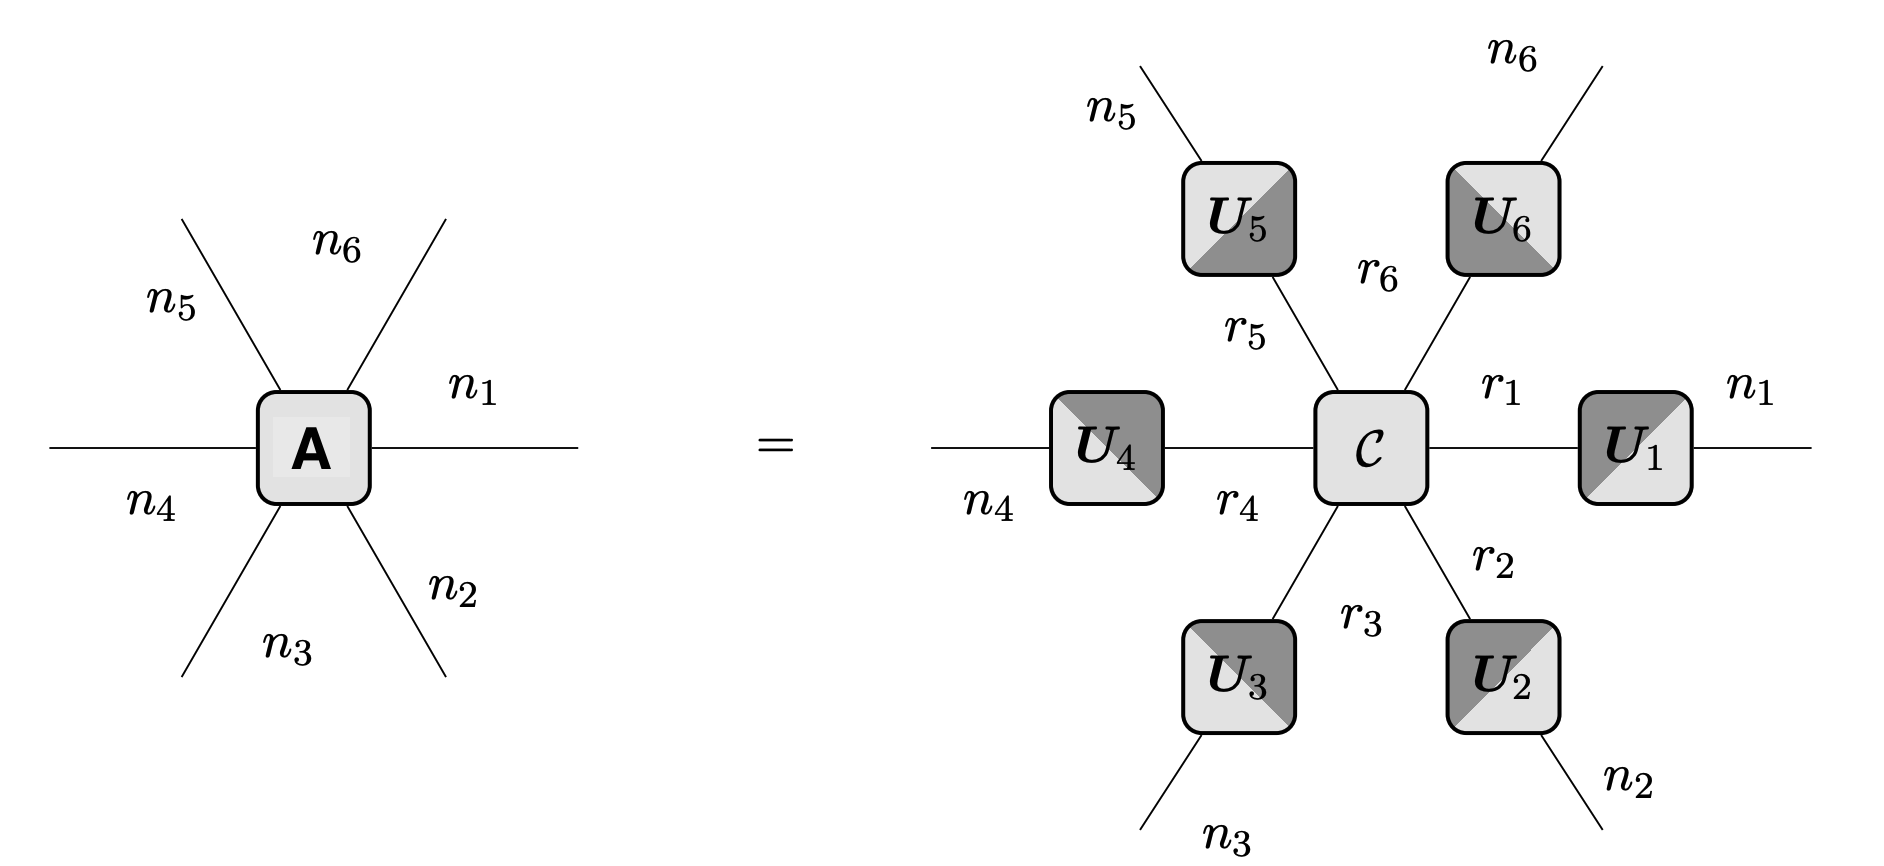
\includegraphics[width=.7\textwidth]{Graphics/TuckerDecomp.png}
\end{figure}
\end{itemize}
Storage of Tucker format: \\
T-rank: 
}

\only<6>{
\begin{itemize}
    \bitem Tucker decomposition:
    Let $\vA \in \mathbb{R}^{n_1\times ... \times n_d}$. Then
 
\begin{figure}
    \centering
    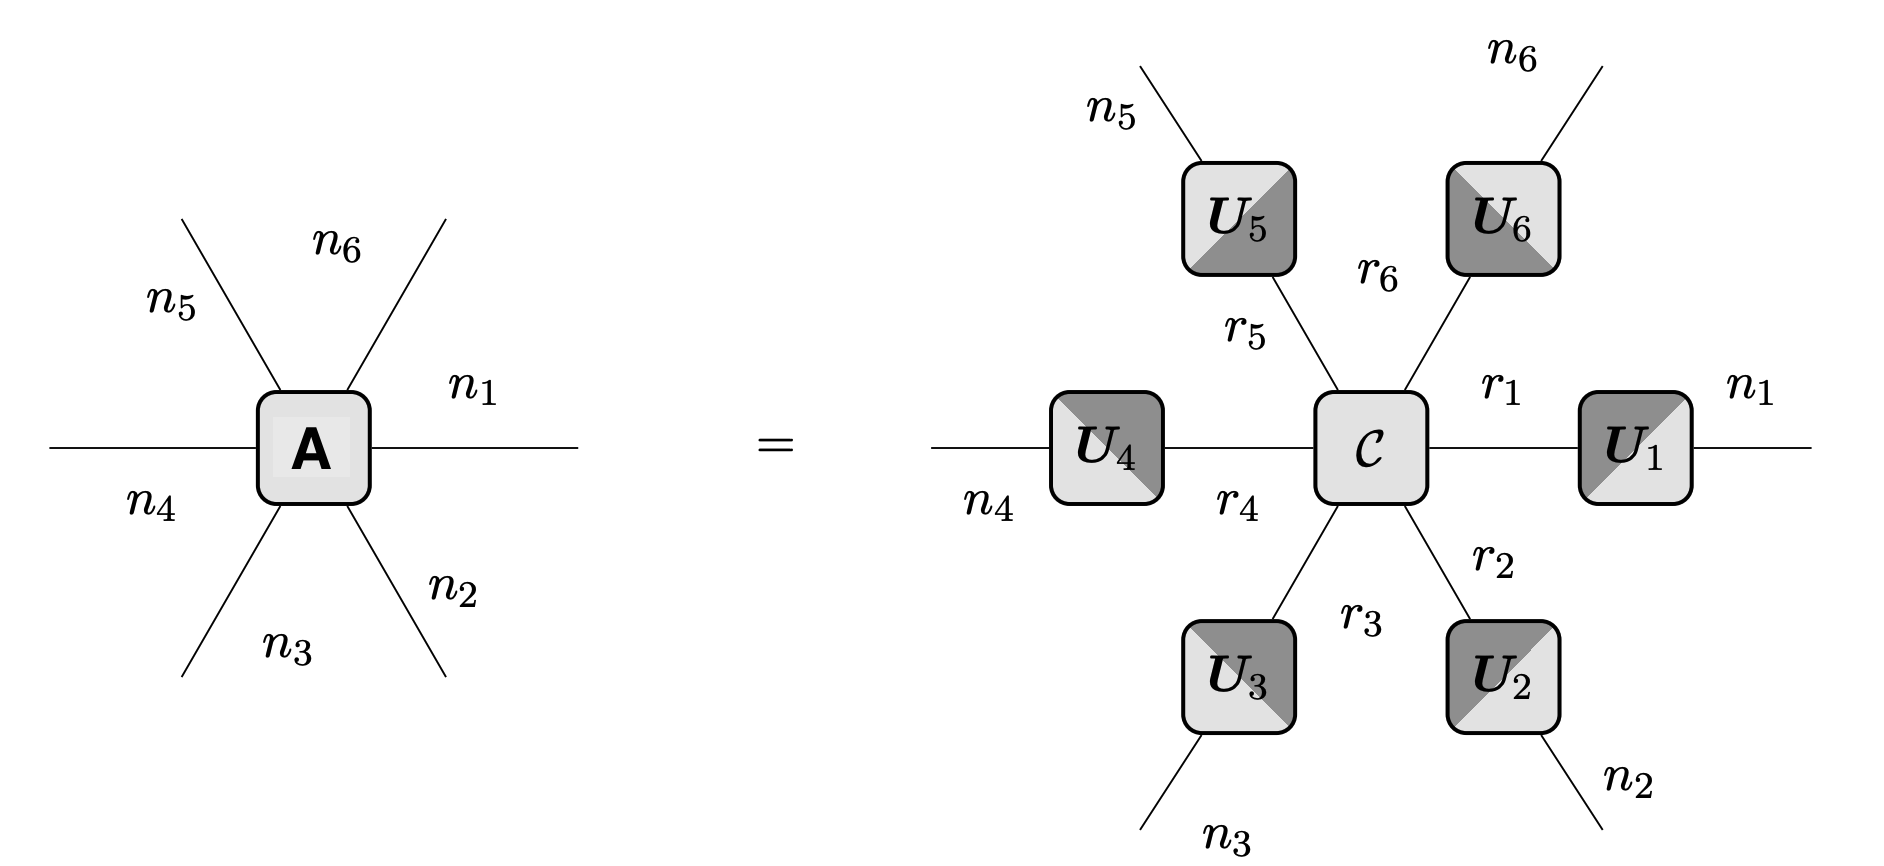
\includegraphics[width=.7\textwidth]{Graphics/TuckerDecomp.png}
\end{figure}
\end{itemize}
Storage of Tucker format: $\mathcal{O}(r^d + rnd)$\\
T-rank: $\vr = (r_1,...,r_d)$\\
Advantage:\vspace{3cm}
}


\only<7>{
\begin{itemize}
    \bitem Tucker decomposition:
    Let $\vA \in \mathbb{R}^{n_1\times ... \times n_d}$. Then
 
\begin{figure}
    \centering
    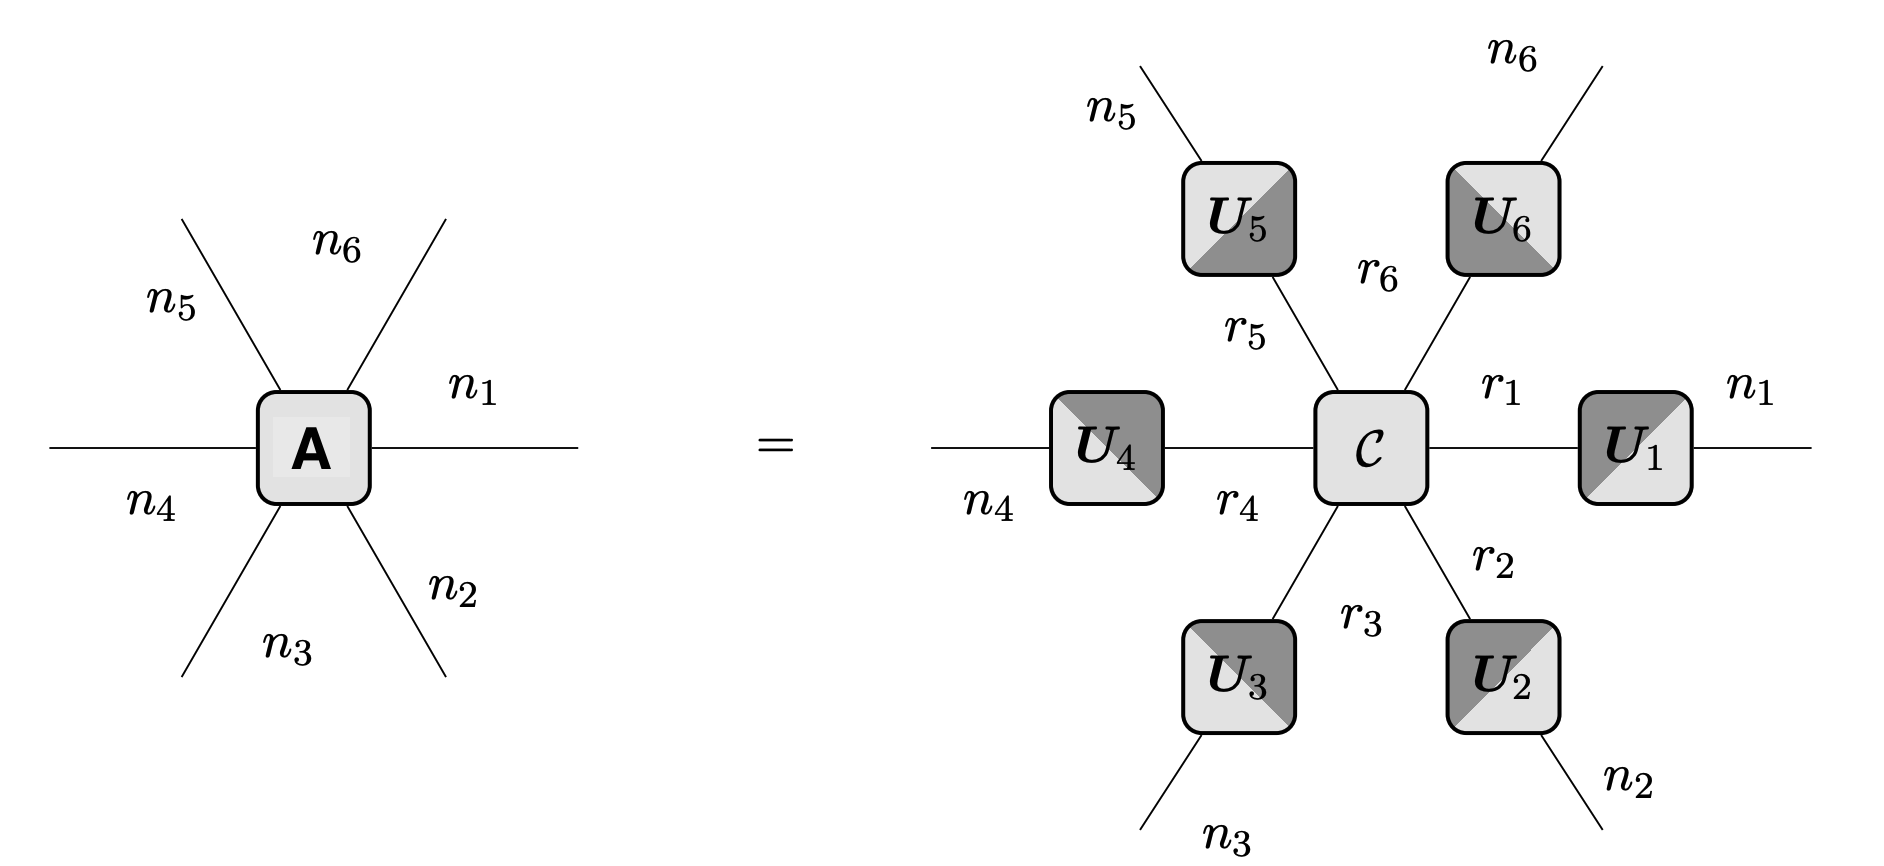
\includegraphics[width=.7\textwidth]{Graphics/TuckerDecomp.png}
\end{figure}
\end{itemize}
Storage of Tucker format: $\mathcal{O}(r^d + rnd)$\\
Advantage: 
\begin{itemize}
    \item[1] Can be computed using HOSVD
    \item[2] Closed set of low-rank tensors
    \item[3] Manifold structure on the set of tensors with fixed rank
    \item[4] Can be sketched
\end{itemize}

}
\end{frame}


\begin{frame}{Recall TT format}


\begin{itemize}
    \bitem TT decomposition: Let $\vA \in \mathbb{R}^{n_1\times ... \times n_d}$. Then
    $$
    \begin{aligned}
    \vA
    &= \vU_1 \circ \vU_d \circ ... \circ \vU_d\\
    &= \vU_1 *_{2,1} \vU_d *_{3,1} ... *_{3,1} \vU_d\\
    &=
    \sum_{k_1 = 1}^{r_1}...\sum_{k_{d-1} = 1}^{r_{d-1}} 
    \vU_1[:,k_1] \vU_2[k_1,:,k_2]  \cdots  \vU_{d-1}[k_{d-2},:,k_{d-1}] \vU_d[k_{d-1},:]
    \end{aligned}
    $$
    \only<2>{
    or elementwise
    \begin{footnotesize}
    $$
    \begin{aligned}
    &\vA[i_1,...,i_d]\\
    &=
    \sum_{k_1 = 1}^{r_1}...\sum_{k_{d-1} = 1}^{r_{d-1}} 
    \vU_1[i_1,k_1] \vU_2[k_1,i_2,k_2]  \cdots  \vU_{d-1}[k_{d-2},i_{d-1},k_{d-1}] \vU_d[k_{d-1},i_d]
    \end{aligned}
    $$
    \end{footnotesize}
    } 
    \only<3>{
    or in diagrams
    \begin{figure}
    \centering
    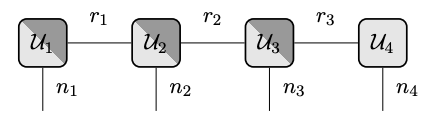
\includegraphics[width = .5\textwidth]{Graphics/TTDecomposition.png}
    \end{figure}
    }
\end{itemize}

\end{frame}

\begin{frame}{TT-SVD}

$$
\begin{aligned}
&\vA_{n_1,...,n_d}\\
\pause
&=
\vA_{n_2\cdots n_d}^{n_1} &&\text{reshape to}~n_1 \times \prod_{j\neq i} n_j\\ \pause
&=
\left(\vU_1\right)_{r_1}^{n_1} (\bSigma_1 \vV_1^\top)_{n_2\cdots n_d}^{r_1}&&\text{SVD}\\ \pause
&=
\left(\vU_1\right)_{r_1}^{n_1}
(\bSigma_1\vV_1^\top)_{n_3\cdots n_d}^{r_1 \cdot n_2}&&\text{reshape of}~ (\bSigma_1\vV_1^\top)\\ \pause
&=
\left(\vU_1\right)_{r_1}^{n_1}
\left(\vU_2\right)^{r_1 \cdot n_2}_{r_2} 
(\bSigma_2\vV_2^\top)_{n_3\cdots n_d}^{r_2}&&\text{SVD of}~ (\bSigma_1\vV_1^\top)\\ \pause
&=
\left(\vU_1\right)_{r_1}^{n_1}
\left(\vU_2\right)^{r_1 \cdot n_2}_{r_2} 
(\bSigma_2\vV_2^\top)_{n_4\cdots n_d}^{r_2\cdot n_3 }&&\text{reshape of}~ (\bSigma_2\vV_2^\top)\\ \pause
&=
\left(\vU_1\right)_{r_1}^{n_1}
\left(\vU_2\right)^{r_1 \cdot n_2}_{r_2}
\left(\vU_3\right)^{r_2 \cdot n_3}_{r_3}
(\bSigma_3\vV_3^\top)_{n_4\cdots n_d}^{r_3}&&\text{SVD of}~ (\bSigma_2\vV_2^\top)\\ \pause
&~~\vdots\\
&=
\underbrace{\left(\vU_1\right)_{r_1}^{n_1}}_{\vU_1[n_d]}
\cdots
\underbrace{\left(\vU_{d-1}\right)^{r_{d-2} \cdot n_{d-1}}_{r_{d-1}}}_{=:\vU_{d-1}[n_{d-1}]}
\underbrace{(\bSigma_{d-1}\vV_{d-1}^\top)_{n_d}^{r_{d-1}}}_{=:\vU_{d}[n_d]}
\end{aligned}
$$
    
\end{frame}


\begin{frame}{HT decomposition}

\begin{itemize}
    \bitem Similar idea as TT format:\\ 
    $\rightarrow$ instead of using the nested subspace use a hierarchy of subspaces 
    \bitem  Define a partition tree for the set of mode indices: \\
    $\rightarrow$ the root of the tree contains the complete set \\ 
    $\rightarrow$ each leaf contains a single mode index\\ 
    $\rightarrow$ each inner node of the tree contains the union of its children
\end{itemize}
    
\end{frame}

\begin{frame}{Tree tensor network}

\begin{center}
What is a partition tree for the set of mode indices?
\end{center}
\pause
\begin{itemize}
    \bitem It is a hierarchical tree 
    \bitem TT format:\\
    ~\\
    \begin{minipage}{4cm}
    \begin{itemize}
        \item[] $\mathbb{R}^{n_1\times n_2 \times n_3 \times n_4}$
        \vspace{4mm}
        \item[] $U_1\otimes \mathbb{R}^{n_2 \times n_3 \times n_4}$ \vspace{5mm}
        \item[] $U_2\otimes \mathbb{R}^{n_3 \times n_4}$ \vspace{4mm}
        \item[] $U_3\otimes \mathbb{R}^{n_4}$ \vspace{4mm}
    \end{itemize}
    \end{minipage}
    \hspace{6mm}
    \begin{minipage}{4cm}
        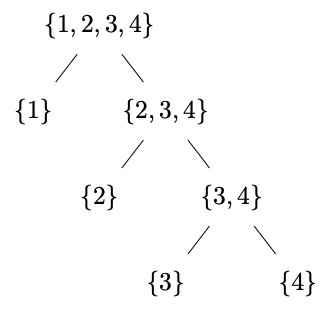
\includegraphics[width =\textwidth]{Graphics/TTTensorTree.png}
    \end{minipage}
    \hfill
\end{itemize}



    
\end{frame}




\begin{frame}{Balanced tree tensor network}

\begin{itemize}
    \bitem Consider $\vU \in \mathbb{R}^{n_1\times n_2\times n_3 \times n_4}$
    \bitem Balanced tree of mode indices:\\
    ~\\
    \begin{minipage}{7cm}
    \begin{itemize}
        \item[] $\mathbb{R}^{n_1\times n_2 \times n_3 \times n_4}$
        \vspace{3mm}
        \item[] $\tilde U_1\otimes \tilde U_2,\quad \tilde U_1\subseteq \mathbb{R}^{n_1 \times n_2},~\tilde U_2\subseteq \mathbb{R}^{n_3 \times n_4}$  \vspace{5mm}
        \item[] $U_1\otimes U_2 \otimes U_3 \otimes U_4$ \vspace{4mm}
    \end{itemize}
    \end{minipage}
    \begin{minipage}{4cm}
    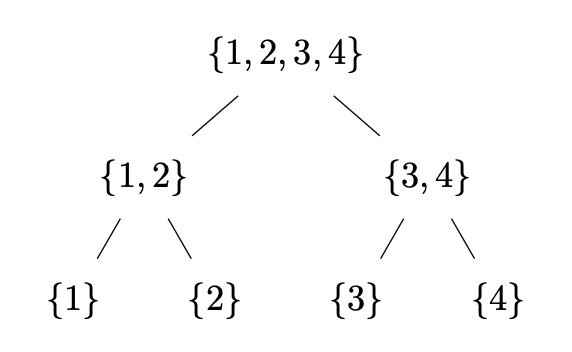
\includegraphics[width = 1.2\textwidth]{Graphics/Balanced_tree.png}
    \end{minipage}
\end{itemize}

\end{frame}

\begin{frame}{Tree tensor networks in diagrams}

\begin{itemize}
    \bitem Compare TT vs HT:\\
    ~\\
    \begin{figure}
        \centering
        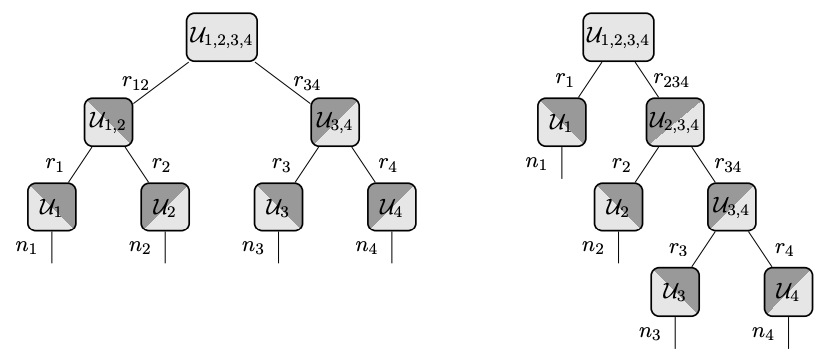
\includegraphics[width = 0.8\textwidth]{Graphics/TuckerVSTT.png}
    \end{figure}
\end{itemize}
    
\end{frame}





\begin{frame}{Recall matricization}

\begin{itemize}
    \bitem For a tensor $\vA \in\mathbb{R}^{n_1\times ... \times n_d}$, a collection of dimension indices $t \subset \{1,...,d\}$, and its complement $s = \{1,...,d\} \setminus t$, we define
    $$
    \vA^{(t)} \in\mathbb{R}^{n_t \times n_s},\quad 
    n_t = \bigtimes_{k \in t}n_k,~n_s = \bigtimes_{k \in s}n_k
    $$
    elementwise defined as
    $$
    [\vA^{(t)}]_{(i_k)_{k\in t},(i_\ell)_{\ell \in s}}
    =
    \vA_{i_1,...,i_d}
    $$
\end{itemize}
    
\end{frame}



\begin{frame}{Matricization example}

\only<1,2>{
Consider
$$
\vA_{i_1, i_2, i_3, i_4}
=
i_1 + 2(i_1 -1 )+ 4(i_3 -1 )+ 8(i_4 -1 ), \quad i_1,i_2,i_3,i_4 \in \{1,2\}
$$
We chose the lexicographical ordering for compound indices
$$
(i_p,...,i_q) \mapsto 
\ell = i_p + n_p(i_{p+1} -1)+ n_pn_{p+1}(i_{p+2} -1) + ... + i_qn_p\cdots n_{q-1}
$$

Compute
$$
\vA^{(\{1\})}
=
\pause
\begin{bmatrix}
1 &3 &5 &7 &9 &11 &13 &15\\
2 &4 &6 &8 &10 &12 &14 &16
\end{bmatrix}
$$
}

\only<3,4>{
Consider
$$
\vA_{i_1, i_2, i_3, i_4}
=
i_1 + 2(i_1 -1 )+ 4(i_3 -1 )+ 8(i_4 -1 ), \quad i_1,i_2,i_3,i_4 \in \{1,2\}
$$
We chose the lexicographical ordering for compound indices
$$
(i_p,...,i_q) \mapsto 
\ell = i_p + n_p(i_{p+1} -1)+ n_pn_{p+1}(i_{p+2} -1) + ... + i_qn_p\cdots n_{q-1}
$$

Compute
$$
\vA^{(\{3\})}
=\pause \pause \pause 
\begin{bmatrix}
1 &2 &3 &4 &9 &10 &11 &12\\
5 &6 &7 &8 &13 &14 &15 &16
\end{bmatrix}
$$
}

\only<5,6>{
Consider
$$
\vA_{i_1, i_2, i_3, i_4}
=
i_1 + 2(i_1 -1 )+ 4(i_3 -1 )+ 8(i_4 -1 ), \quad i_1,i_2,i_3,i_4 \in \{1,2\}
$$
We chose the lexicographical ordering for compound indices
$$
(i_p,...,i_q) \mapsto 
\ell = i_p + n_p(i_{p+1} -1)+ n_pn_{p+1}(i_{p+2} -1) + ... + i_qn_p\cdots n_{q-1}
$$

Compute
$$
\vA^{(\{2,3,4\})}
=\pause \pause \pause \pause \pause 
\begin{bmatrix}
1 &2\\
3 &4\\
5 &6\\
7 &8\\
9 &10\\
11 &12\\
13 &14\\
15 &16
\end{bmatrix}
=
(\vA^{(\{1\})})^\top
$$
}

\end{frame}


\begin{frame}{Matricization Tucker format}

Consider the tensor
$$
\vA=
\begin{bmatrix}
1\\2
\end{bmatrix}
\otimes 
\begin{bmatrix}
3\\4
\end{bmatrix}
\otimes 
\begin{bmatrix}
5\\6
\end{bmatrix}
\pause
=
\left[
\begin{bmatrix}
15 & 20 \\
30 & 40
\end{bmatrix} ,
\begin{bmatrix}
18 & 24\\
36 & 48
\end{bmatrix}
\right]
$$
Then its $(\{1,2\})$-matrizication is 
$$
\begin{aligned}
\vA^{(\{1,2\})}
\pause
&=
\begin{bmatrix}
15 &18\\
30 &36\\
20 &24\\
40 &48
\end{bmatrix}
\pause
&=
\left(
\begin{bmatrix}
1\\2
\end{bmatrix}
\otimes 
\begin{bmatrix}
3\\4
\end{bmatrix}
\right)^{(\{1,2\})}
\cdot
\left(
\left(
\begin{bmatrix}
5\\6
\end{bmatrix}
\right)^{(\{1\})}
\right)^\top
\end{aligned}
$$

\end{frame}

\begin{frame}{Matricization Tucker format}

\only<1,2>{
Consider the tensor $\vA \in \mathbb{R}^{n_1\times n_2\times n_3}$
$$
\vA = \sum_{j_1=1}^{k_1}\sum_{j_2=1}^{k_2}\sum_{j_3=1}^{k_3}
c_{j_1,j_2,j_3} \vu_{j_1,1} \otimes \vu_{j_2,2} \otimes \vu_{j_3,3}
$$
Then
$$
\vA^{(\{1,2\})}
=
\sum_{j_1=1}^{k_1}\sum_{j_2=1}^{k_2}
\left(
\vu_{j_1,1} \otimes \vu_{j_2,2}
\right)^{(\{1,2\})}
\cdot
\left(
\sum_{j_3=1}^{k_3} c_{j_1,j_2,j_3}\vu_{j_3,3}
\right)^\top
$$
}
    
\end{frame}

\begin{frame}{Rank bound}
Lemma:\\
Let $\vA \in \mathbb{R}^{n_1 \times n_2 \times n_3}$ with 
$$
\vA = \sum_{j_1=1}^{k_1}\sum_{j_2=1}^{k_2}\sum_{j_3=1}^{k_3}
c_{j_1,j_2,j_3} \vu_{j_1,1} \otimes \vu_{j_2,2} \otimes \vu_{j_3,3}.
$$
Then
$$
{\rm rank} (\vA^{(\{1,2\})}) \leq \min(\{k_1\cdot k_2, k_3\}).
$$
    
\end{frame}

\begin{frame}{Root-to-leaves truncated hierarchical SVD\footnote{Grasedyck, SIAM Journal on Matrix Analysis and Applications, 2010}}
\begin{footnotesize}
Set $\mathcal{I} = n_1\times ...\times n_d$, and let $T_{\mathcal{I}}$ be a dimension tree of depth $p\in\mathbb{N}$. We call $\mathcal{L}(T_\mathcal{I})$ the leafs of the $T_{\mathcal{I}}$, and $\mathcal{I}(T_\mathcal{I})$ are the internal nodes of the $T_{\mathcal{I}}$.\\
~\\
Algorithm:
\begin{itemize}
    \item[]Input: $\vA \in \mathbb{R}^{\mathcal{I}}$, $T_{\mathcal{I}}$, target rank $(r_t)_{t\in T_{\mathcal{I}}}$
    \item[]Output:  $(\vU_t)_{t\in\mathcal{L}(T_{\mathcal{I}})}$,  $(\vB_t)_{t\in\mathcal{I}(T_{\mathcal{I}})}$
    \item[] for $t\in\mathcal{L}(T_\mathcal{I})$
    \item[] $\qquad$ $\vU_t, \bSigma_t, \vV_t = {\rm SVD}(\vA^{(t)}, r_t)$ 
    \item[] for $\ell = p-1:0$
    \item[] $\qquad$ for $t\in \mathcal{I}(T_\mathcal{I})$ on level $\ell$
    \item[] $\qquad\qquad$ $\vU_t, \bSigma_t, \vV_t = {\rm SVD}(\vA^{(t)}, r_t)$
    \item[] $\qquad\qquad$ $\vU_{t_1}$ and $\vU_{t_2}$ be successors of $t$.
    \item[] $\qquad\qquad$ compute
    $
    (\vB_{t})_{i,j,k} = \langle (\vU_{t_1})_i, (\vU_{t_2})_j \otimes (\vU_{t_1})_k \rangle
    $
    \item[] Compute $
    (\vB_{\{1,...,d\}})_{1,j,k} = \langle (\vA, (\vU_{t_1})_j \otimes (\vU_{t_2})_k \rangle
    $
\end{itemize}
\end{footnotesize}

\end{frame}

\begin{frame}{Hierarcical Tucker format}

Tree tensor network:
$$(\vU_t)_{t\in\mathcal{L}(T_{\mathcal{I}})}
\quad {\rm and}\quad 
(\vB_t)_{t\in\mathcal{I}(T_{\mathcal{I}})}$$
Storage: \pause
$\mathcal{O}(rnd + dr^3)$ \\
~\\
Compare to TT:
$\mathcal{O}(dnr^2)$

\begin{center}
Why HT?
\end{center}
\pause
$\Rightarrow$ Remember, the tensor rank is not uniquely defined!\\~
~\\
A tensor $\vA$ may be {\it exactly} represented in HT and TT format, however, the ranks appearing in HT can be lower!\\
(Consequence of general rank bounds\footnote{Grasedyck \& Hackbusch, Computational Methods in Applied Mathematics, 2011})
\end{frame}


\end{document}




